\begin{frame}
  \frametitle{Un teorema di tipo ``Wolff-Denjoy'' per sottovarietà relativamente compatte}
  \only<1-2>{
    \begin{defn}
      Una varietà complessa $X$ si dice \textit{taut} se ogni funzione nella chiusura (rispetto alla topologia compatta-aperta) di $\text{Hol}(\mathbb{D},X)$ in $C^0(\mathbb{D},X^*)$ è in $\text{Hol}(\mathbb{D},X)$ oppure è la funzione costante $\infty$.
  \end{defn}\pause

    Si può dimostrare che ogni varietà taut è Kobayashi-iperbolica.
  }
  \only<3->{
    \begin{block}{Teorema (Chandel, Maitra, Sarkar, 2021; Bharali, Zimmer, 2022)}\begin{itshape}
      Sia $X$ una sottovarietà taut e relativamente compatta di una varietà complessa $Y$. \setcounter{beamerpauses}{3}\pause Supponiamo che esista un $\kappa_0>0$ tale che $X$ sia $(1,\kappa_0)$-visibile.
    
      Sia $F:X \longrightarrow X$ una funzione olomorfa. \pause Allora vale esattamente una delle seguenti affermazioni: \pause
      \begin{itemize}
        \item le orbite dei punti di $X$ tramite $F$ sono relativamente compatte in $X$; \pause oppure,
        \item esiste un unico punto di $\partial_YX$ tale che la successione delle iterate di $F$ converge, uniformemente sui compatti, a quel punto.
      \end{itemize}
    \end{itshape}\end{block}
  }
\end{frame}

\begin{frame}
  \frametitle{Un esempio di Bharali e Maitra: i domini Caltrops}
  \only<1-3>{
    \begin{defn}
      Un dominio limitato $\Omega\subseteq\mathbb{C}^n$, con $n\ge 2$, è detto \textit{dominio Caltrop} se esiste un insieme finito di punti $\{q_1,\dots,q_N\}\subseteq\partial\Omega$ tale che:\pause
      \begin{itemize}
          \item il sottoinsieme del bordo $\partial\Omega\setminus\{q_1,\dots,q_N\}$ è $C^2$ e $\Omega$ è strettamente pseudoconvesso in ogni punto di tale insieme;\pause
          \item per ogni $j=1,\dots, N$ esistono un intorno aperto e connesso $V_j\ni q_j$, due costanti $p_j\in(1,3/2)$ e $C_j>1$, una trasformazione unitaria $\mathbb{U}^{(j)}$ e una funzione continua $\psi_j:[0,A_j]\longrightarrow[0,+\infty)$, con $A_j>0$, tali che $\mathbb{U}_j(\Omega\cap V_j)$ è un ``solido di rivoluzione'':
      \end{itemize}
    \end{defn}
  }
  \only<4-9>{
    \begin{defn}
      \begin{equation*}\begin{split}
        \mathbb{U}_j(\Omega\cap V_j)=&\Bigg\{(z_1,\dots,z_n)\in\mathbb{C}^n\mid \mathfrak{Re}z_n\in (0,A_j),\\
        &(\mathfrak{Im}z_n)^2+\sum_{j=1}^{n-1}|z_j|^2<\psi_j(\mathfrak{Re}z_n)^2\Bigg\}
      \end{split}\end{equation*}
      dove $\mathbb{U}_j(z)=\mathbb{U}^{(j)}(z-q_j)$ per ogni $z\in\mathbb{C}^n$. \setcounter{beamerpauses}{4}\pause Inoltre, $\psi_j$ ha le seguenti proprietà:\pause
      \begin{itemize}
        \item è di classe $C^2$ su $(0,A_j)$;\pause
        \item per ogni $x\in[0,A_j]$ si ha $(1/C_j)x^{p_j} \le \psi_j(x) \le C_jx^{p_j}$;\pause
        \item si ha che $\psi_j$ è strettamente crescente e $\psi_j'$ è crescente su $(0,A_j)$;\pause
        \item si ha $\displaystyle\lim_{x\longrightarrow0^+}\psi_j(x)\psi_j''(x)=0$.
      \end{itemize}
    \end{defn}
  }
  \only<10>{
    \begin{figure}
      \begin{center}
          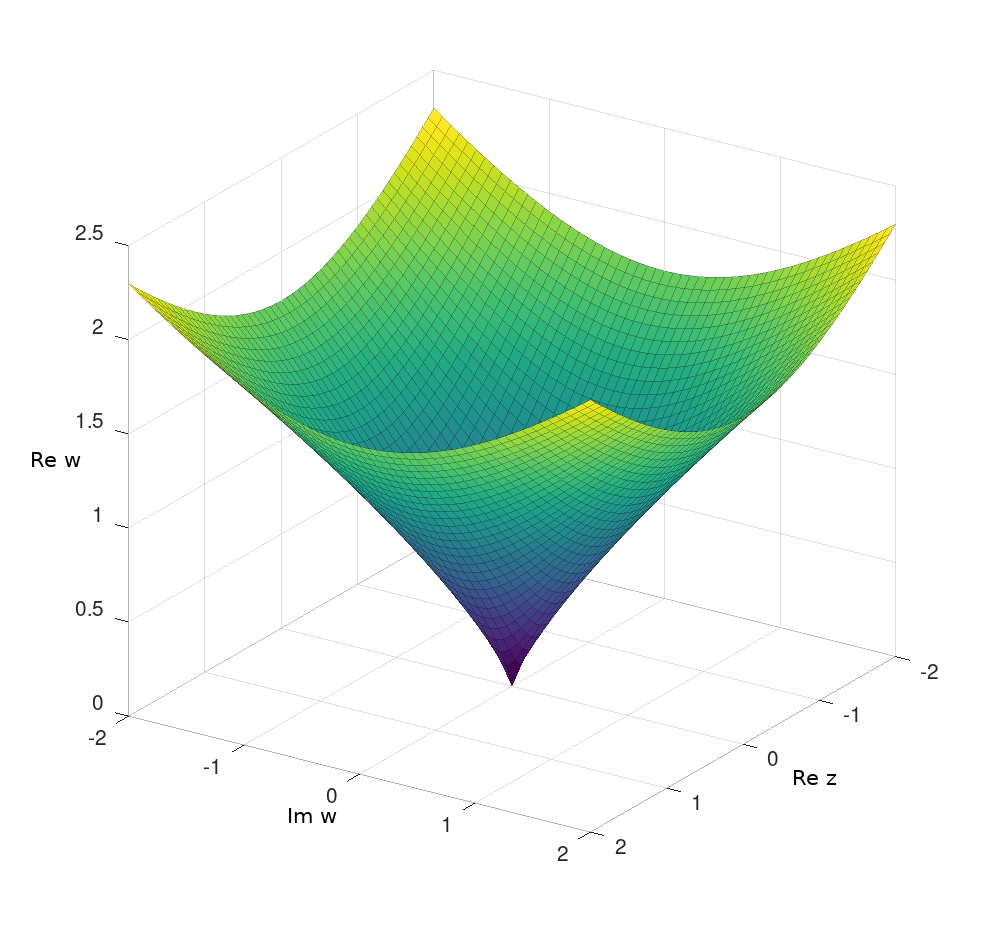
\includegraphics[width=0.65\textwidth, trim=0 4cm 0 1.7cm]{caltrop.png} \\
          \caption{proiezione a $\mathfrak{Im}z=0$ del bordo della punta in $\mathbb{C}^2$ con coordinate $(z,w)$ corrispondente a $\psi(x)=x^{5/4}$}
      \end{center}
  \end{figure}
  }
\end{frame}

\begin{frame}{Costruzione di un dominio Caltrop in $\mathbb{C}^2$}
  Siano $A,\beta>0$ e sia $\psi:[-A,\beta]\longrightarrow[0,+\infty)$ una funzione continua di classe $C^2$ su $(-A,\beta)$ tale che:\pause
  \begin{enumerate}
    \item per ogni $t\in(-A,-B)$ si ha $\psi(t)=(t+A)^p$;\pause
    \item per ogni $t\in(0,\beta)$ si ha $\psi(t)=\sqrt{\beta^2-t^2}$,
  \end{enumerate}
  dove $B\in(0,A)$ e $p\in(1,3/2)$. \pause Il dominio cercato è
  $$\Omega:=\{(z,w)\in\mathbb{C}^2\mid |z|^2+|\mathfrak{Im}w|^2<C\psi(\mathfrak{Re}w)^2,-A<\mathfrak{Re}w<\beta\},$$
  dove $C>0$ è una costante opportunamente scelta.\pause
  
  Le verifiche necessarie seguono da come è definita $\psi$; \pause per la pseudoconvessità, la funzione di definizione è
  $$\rho(z,w):=|z|^2+|\mathfrak{Im}w|^2-C\psi(\mathfrak{Re}w)^2.$$
\end{frame}

\begin{frame}[t]{I domini Caltrops sono $(\lambda,\kappa)$-visibili}
  \only<1-7>{
    Sia $\Omega$ un dominio limitato di $\mathbb{C}^d$. Poniamo
    $$M_\Omega(r):=\sup\left\{\frac{1}{K_\Omega(x;v)}\mid x\in\Omega,\delta_\Omega(x) \le r, \|v\|=1\right\},$$
    dove $\delta_\Omega$ indica la distanza euclidea da $\partial\Omega$.\pause
    \begin{block}{Teorema (Bharali, Maitra, 2021)}\begin{itshape}
      Sia $\Omega$ un dominio limitato di $\mathbb{C}^d$. \setcounter{beamerpauses}{2}\pause Supponiamo che esistano uno $z_0\in\Omega$ e una funzione $C^1$ strettamente crescente $f:(0,+\infty)\longrightarrow\mathbb{R}$, con $f(t)\longrightarrow+\infty$ per $t\longrightarrow+\infty$, tali che:\pause
      \begin{enumerate}
          \item si ha $k_\Omega(z_0,z) \le f\big(1/\delta_\Omega(z)\big)$ per ogni $z\in\Omega$;\pause
          \item si ha $M_\Omega(r)\longrightarrow 0$ per $r\longrightarrow 0$;\pause
          \item esiste $r_0>0$ tale che $\displaystyle\int_0^{r_0}\frac{M_\Omega(r)}{r^2}f'\left(\frac{1}{r}\right)\diff r<+\infty$.
      \end{enumerate}\pause
        
      Allora $\Omega$ è $(\lambda,\kappa)$-visibile per ogni $\lambda \ge 1$ e $\kappa>0$.
    \end{itshape}\end{block}
  }
  \only<8->{
    \begin{prop}
      I domini Caltrops sono $(\lambda,\kappa)$-visibili per ogni $\lambda\ge 1$ e $\kappa>0$.
    \end{prop}\setcounter{beamerpauses}{8}\pause
    \textit{Idea della dimostrazione:} si usa il teorema di Bharali e Maitra. Per vedere che un dominio Caltrop $\Omega$ ne soddisfa le ipotesi: \pause si calcola $k_D$ per un certo dominio planare $D$ usato come modello; \pause dopodiché si immergono copie di $D$ in $\Omega$ in maniera affine, di modo che ogni punto di $\Omega$ sufficientemente vicino al bordo sia contenuto in una di queste copie; \pause a questo punto, si usa il fatto che le funzioni olomorfe sono contrazioni per $k_X$ per stimare la distanza di Kobayashi su $\Omega$.
  }
\end{frame}

\begin{frame}{I domini Caltrop sono taut}
  \only<1->{
    \begin{lemma}
      Ogni varietà $X$ Kobayashi-iperbolica e $k_X$-completa è taut.
    \end{lemma}\pause
    \begin{lemma}
      Sia $\Omega\subseteq\mathbb{C}^n$ un dominio limitato tale che esiste uno $z_0\in\Omega$ tale che per ogni $\xi\in\partial\Omega$ si ha $\displaystyle\lim_{w\longrightarrow\xi}k_\Omega(z_0,w)=+\infty$; allora $(\Omega,k_\Omega)$ è completo.
    \end{lemma}\pause
    \begin{prop}
      I domini Caltrops sono taut.
    \end{prop}\pause
    \textit{Idea della dimostrazione:} Si usano i Lemmi. Si distinguono due casi.\pause

    $\xi\in\partial\Omega\setminus\{q_1,\dots,q_N\}$: si usa la pseudoconvessità;\pause

    $\xi=q_j$ per $j=1,\dots,N$: si usa la forma di $\Omega$ vicino a $q_j$.
  }
\end{frame}

\begin{frame}
  \frametitle{Strada per la dimostrazione del teorema di tipo ``Wolff-Denjoy''}
  \begin{enumerate}
    \item dall'ipotesi che la varietà sia taut, per un teorema di Abate segue che se le orbite non sono relativamente compatte allora la successione delle iterate è compattamente divergente;\pause
    \item dalle ipotesi di visibilità e di relativa compattezza segue, a meno di sottosuccessioni, la convergenza uniforme sui compatti a una costante nel bordo della varietà;\pause
    \item sempre per la condizione di visibilità, tale limite è lo stesso per ogni sottosuccessione, dunque dev'essere il limite di tutta la successione.
  \end{enumerate}
\end{frame}